%    2. Write your answers in section "B" below. Precede answers for all 
%       parts of a question with the command "\question{n}{desc}" where n is
%       the question number and "desc" is a short, one-line description of 
%       the problem. There is no need to restate the problem.
%    3. If a question has multiple parts, precede the answer to part x with the
%       command "\part{x}".
%    4. If a problem asks you to design an algorithm, use the commands
%       \algorithm, \correctness, \runtime to precede your discussion of the 
%       description of the algorithm, its correctness, and its running time, respectively.
%    5. You can include graphics by using the command \includegraphics{FILENAME}
%
\documentclass[11pt]{article}
\usepackage{amsmath,amssymb,amsthm}
\usepackage{graphicx}
\usepackage[margin=1in]{geometry}
\usepackage{fancyhdr}
\usepackage{float}
\newcommand\ceil[1]{\lceil#1\rceil}
\setlength{\parindent}{0pt}
\setlength{\parskip}{5pt plus 1pt}
\setlength{\headheight}{13.6pt}
\newcommand\question[2]{\vspace{.25in}\hrule\textbf{#1}\vspace{.5em}\hrule\vspace{.10in}}
\renewcommand\part[1]{\vspace{.10in}\textbf{(#1)}}
\pagestyle{fancyplain}
\lhead{\textbf{\NAME\ (\UID)}}
\chead{\textbf{Optimization and Online Learning}}
\rhead{CS 6966, \today}
\begin{document}\raggedright

\newcommand\NAME{Jake Pitkin}
\newcommand\UID{u0891770}
\newcommand\HWNUM{2}

\question{Problem 6 - Convexity Basics}

For this problem, let $f$ be a convex function defined over a convex set $K$, and suppose the diameter of $K$ is $1$.

\part{a} Let $x \in K$, and suppose $f(x) = 2$ and $\vert \vert \nabla f(x) \vert \vert = 1$. Give a lower bound on min$_{z \in K}$ $f(z)$.

\fbox{ \parbox{1\linewidth}{

} }

\part{b} Let $x^*$ be the minimizer of $f$ over $K$ (suppose it is unique), and let $x$ be any other point. The intuition behind gradient descent is that the vector: $- \nabla f(x)$ points \textit{towards} $x^*$. Prove that this is indeed true, in the sense that $\langle \nabla f(x), x - x^* \rangle \geq 0$ (i.e., the negative gradient makes an acute angle with the line to the optimum).

\fbox{ \parbox{1\linewidth}{

From the lecture 7 scribe notes we have the following property of convex functions

$$f(y) - f(x) \geq \langle y - x, \nabla f(x) \rangle \ \ \forall x, y$$

We will apply this property to a unique $x^* \in K$ and any other point $x \in K$

$$f(x^*) - f(x) \geq \langle x^* - x, \nabla f(x) \rangle $$

Our goal is to show $\langle \nabla f(x), x - x^* \rangle \geq 0$, so we will multiply both sides by $-1$ to change the direction of the inequality

$$- \langle x^* - x, \nabla f(x) \rangle \geq f(x) - f(x^*)$$

Applying the commutative property of dot products and distributing the negative gives us

$$\langle \nabla f(x), x - x^* \rangle \geq f(x) - f(x^*)$$

We know that $x^*$ is a minimizer of $f$ over $K$, it follows that

$$f(x) - f(x^*) \geq 0 \ \ \forall x \in K$$

Thus we have shown that $\langle \nabla f(x), x - x^* \rangle \geq 0$, proving the vector $- \nabla f(x)$ points \textit{towards} $x^*$ for all $x \in K$.

} }

\part{c} Suppose now that the function $f$ is \textit{strictly convex} i.e., $f(\lambda x + (1 - \lambda) y) < \lambda f(x) + (1 - \lambda) f(y)$ (strictly), for all $x \neq y$, and $0 < \lambda < 1$. Prove that all the \textit{maximizers} of $f$ over $K$ lie on the boundary of $K$. [\textit{Hint:} You many want to use the definition that a point $x$ is not on the boundary iff there exists points $y, z \in K$ such that $x = (y + z)/2$.]

\fbox{ \parbox{1\linewidth}{

\textit{proof by contradiction:} Let's $x \in K$ be a \textit{maximizer} of $f$ and assume that $x$ is \textbf{not} on the boundary of $K$. \\

Take $y, z \in K$ such that $y \neq z$ and $x = (y + z) / 2$. We know $y, z \in K$ exist as $x$ is not on the boundary and using the provided hint. Since $x$ is a \textit{maximizer} of $f$, then it follows that $f(x) \geq f(y)$ and $f(x) \geq f(z)$. Applying the definition of \textit{strictly convex} to $y$ and $z$

$$f(\lambda y + (1 - \lambda) z ) < \lambda f(y) + (1 - \lambda) f(z)$$

Using $f(x) \geq f(y)$ and $f(x) \geq f(z)$ we can give an upper-bound

$$f(\lambda y + (1 - \lambda) z ) < \lambda f(y) + (1 - \lambda) f(z) \leq f(x)$$

Ignoring the middle term gives us

$$f(\lambda y + (1 - \lambda) z ) < f(x)$$

We know that $x = (y + z) / 2$. By making this substitution for $x$ and taking $\lambda = 1/2$

$$f(\frac{y}{2} + \frac{z}{2}) < f(\frac{y + z}{2})$$
$$f(\frac{y + z}{2}) < f(\frac{y + z}{2})$$

We arrive at a contradiction as the inequality is strict. Thus all the \textit{maximizers} of $f$ over $K$ lie on the boundary of $K$.

} }

\question{Problem 7 - Gradient Descent Basics}

\part{a} Give an example of a function defined over $\mathbb{R}$, for which for \textit{any} step-size $\eta > 0$ (no matter how small), gradient descent with step-size $\eta$ oscillates around the optimum point (i.e., never gets to distance $< \eta/4$ to it), for some starting point $x \in \mathbb{R}$.

\fbox{ \parbox{1\linewidth}{
Consider the absolute value function $g(x) = |x|$ defined over $\mathbb{R}$.

\begin{figure}[H]
  \centerline{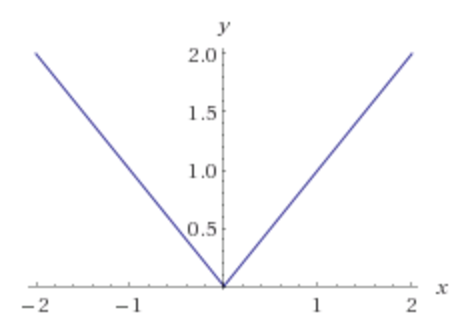
\includegraphics[width=0.4\linewidth]{abs.png}}
\end{figure}

The absolute value function is convex but it is not smooth. It is not differentiable as the derivative at $x = 0$ is not defined. For any arbitrarily small step-size $\eta$, we can find a starting point $x \in \mathbb{R}$ such that gradient descent will oscillate around the optimum point (never getting to distance $< \eta /4$ to it). \\

Each iteration gradient descent takes a step in the direction of the negative gradient at the current point, with a step-size of $\eta$.

$$\mathbf{w}^{(t + 1)} = \mathbf{w}^{(t)} - \eta \nabla g(\mathbf{w}^{(t)})$$

The $\nabla g(x)$ is defined as

$$
\nabla g(x) = \left\{
        \begin{array}{ll}
            -1 & \quad x < 0 \\
            undefined & \quad x = 0 \\
            1 & \quad x > 0
        \end{array}
    \right.
$$

As such, we can see at each iteration of gradient descent we will take a $ \eta$ sized step from the current point. This step will be in the positive direction if $x$ is negative and vice-versa. For example take the starting point $x = \eta / 2$. At each iteration of gradient descent, we will oscillate between $x = - \eta / 2$ and $x = \eta / 2$. Thus we will never get within $\eta / 4$ of the optimum.

} }

\part{b} Consider the function $f(x, y) = x^2 + \frac{y^2}{4}$, and suppose we run gradient descent with starting point $(1, 1)$, and $\eta = 1/4$. Do we get arbitrarily close to the minimum? Experimentally, find the \textit{threshold} for $\eta$, beyond which the gradient descent starts to oscillate.

\fbox{ \parbox{1\linewidth}{
Given the function $f(x, y) = x^2 + \frac{y^2}{4}$ with a starting point of $\mathbf{w}^{(1)} = (1, 1)$ and $\eta = 1/4$ we get arbitrarily close to the minimum. The minimum of $f(x, y)$ is 0 when $\mathbf{w} = (0, 0)$. To explore this gradient descent scenario, I wrote a program to calculate $\mathbf{w}^{(t)}$ and defined arbitrarily close to being within $0.0001$ of the minimum. I found after 39 steps that $\mathbf{w}^{(39)} = (3.6379\mathrm{e}{-12}, 0.0063)$ and $f(x, y) = 9.7848\mathrm{e}{-06}$. Given enough iterations, the gradient descent found the optimum point (barring floating-point precision issues). \\

Using a program, I found the threshold for $\eta$. I found that gradient descent does not find the optimum point when $\eta \geq 1$. When $\eta = 1$, the behavior is interesting. The $x$ component of $\mathbf{w}^{(t)}$ alternates between the values $1$ and $-1$ and the $y$ component converges to $0$. As such, $f(x, y) = 1$ which is not arbitrarily close to the minimum.
} }

\part{c} Why is the behavior similar to that in part (a) (oscillation for every $\eta$) not happening in part (b)?

\fbox{ \parbox{1\linewidth}{
In part (a) we observed that the absolute value function $g(x) = |x|$ oscillates around the optimum point despite choosing an arbitrarily small step-size $\eta$. In part (b) we concluded that $f(x, y) = x^2 + \frac{y^2}{4}$ with reach the optimum point given a step-size $\eta < 1$. \\

If we consider the gradient of $f(x, y)$ which is defined as 

$$\nabla f(x, y) = (2x, \frac{y}{2})$$

and the update for each iteration of gradient descent

$$\mathbf{w}^{(t + 1)} = \mathbf{w}^{(t)} - \eta \nabla f(\mathbf{w}^{(t)})$$

We can observe that $\mathbf{w}^{(t + 1)}$ is dependent on the value of $x_t$, $y_t$, and a fixed $\eta$. As $x_t$ and $y_t$ get closer to 0, the update "size" at each iteration decreases (since $\vert \vert \nabla f(x, y) \vert \vert$ decreases). This was not the case with $g(x)$, as the direction of the update is dependent on $x$ but the "size" of the update is only dependent on $\eta$. Thus, with a reasonably small $\eta$, $f(x, y)$ will reach the optimum point.

} }

\question{Problem 8 - Stochastic Gradient Descent}

Suppose we have points $(a_1, b_1), (a_2, b_2), ... , (a_n, b_n)$ in the plane and suppose that $\vert a_i \vert \leq 1$, and $\vert b_i \vert \leq 1$ for all $i$. Let $f(x, y) = \frac{1}{n} \sum_{i = 1}^n f_i(x, y)$, where $f_i(x, y) = (x - a_i)^2 + (y - b_i)^2$.

\part{a} What is the point $(x , y)$ that minimizes $f(x, y)$?

\fbox{ \parbox{1\linewidth}{

We can observe that $f_i(x, y) = (x - a_i)^2 + (y - b_i)^2$ is minimized when $x = a_i$ and $y = b_i$. This is true as $f_i(x = a_i, y = b_i) = 0$ for all $\vert a_i \vert \leq 1$ and $\vert b_i \vert \leq 1$ and $f_i(x, y)$ is a non-negative function. \\

The intuition is we want to minimize the average distance from a point $(x, y)$ to each point $(a_i, b_i)$ from the sampled $(a_1, b_1), (a_2, b_2), ... , (a_n, b_n)$ points in the plane. This is from an observation that $f_i(x, y)$ is minimized the closer $x - a_i$ and $x - b_i$ are to zero. To find the point $(x, y)$ that minimizes $f(x, y)$, we take

$$x = \frac{1}{n} \sum_{i = 1}^n a_i \ \ \ \ \ \ \ \ \ y = \frac{1}{n} \sum_{i = 1}^n b_i$$

or the average value of the $n$ sampled $a_i$ and $b_i$.

} }

\part{b} Suppose we perform gradient descent (on $f$) with step size $0 < \eta < 1$. Give the geometric interpretation for one iteration.

\fbox{ \parbox{1\linewidth}{

} }

\part{c} Now suppose we perform stochastic gradient descent with fixed step-size $0 < \eta < 1$, and by picking $i$ at random in $\{1, ... , n\}$, and moving along the gradient of $f_i$ (as in SGD seen in class). After $T$ steps, for $T$ large enough, can we say that we get arbitrarily close to the optimum? (Provide a clear explanation). [\textit{Hint:} Remember $\eta$ is fixed.]

\fbox{ \parbox{1\linewidth}{

} }

\part{d} Pick $n = 100$ random points in $[-1, 1]^2$ (uniformly), and run SGD for fixed $\eta = 1/2$, as above. Write down what the distance to optimum is, after $T = 10$, $T = 100$, and $T = 1,000$ iterations (if you want to be careful, you should average over 5 random choices for the initialization). Now consider dropping step size $\eta_t = 1/t$, and write down the result for $T$ as above.

\fbox{ \parbox{1\linewidth}{

\textbf{Experiment 1:} I ran SGD with 100 random points in $[-1, 1]^2$ and a fixed $\eta = 1/2$. I randomly initialized $(x, y)$ in $[-100000, 100000]^2$ and took an average of the distance from the optimum point (keeping the same 100 random points for each instance).

 \begin{table}[H]
\centering
{\renewcommand{\arraystretch}{1.2}%
\begin{tabular}{| c | c |}
\hline
t & distance\\
\hline
10 & 0.005107\\ \hline
100 & 0.005202\\ \hline
1,000 & 0.00495\\ \hline
\end{tabular}}
\caption{Results at $t = 10, 100$, and $1,000$ for a fixed $\eta$.}
\end{table}

\textbf{Experiment 2:} Same as in experiment 1 but now at each iteration $\eta$ is updated such that $\eta_t = 1/t$.

\begin{table}[H]
\centering
{\renewcommand{\arraystretch}{1.2}%
\begin{tabular}{| c | c |}
\hline
t & distance\\
\hline
10 & 0.00166\\ \hline
100 & 0.0003\\ \hline
1,000 & 0.000009\\ \hline
\end{tabular}}
\caption{Results at $t = 10, 100$, and $1,000$ for $\eta_t = 1/t$.}
\end{table}

We can observe in experiment 1 we experience oscillation around the optimum point when $\eta$ is fixed at $1/2$. Alternatively, if we decrease the step-size at each iteration it allows us to get arbitrarily close to the optimum point.

} }

\question{Problem 9 - Numeric Accuracy in MW Updates}

Consider the randomized experts setting we saw in class (we maintain a distribution over experts at each time, and the loss of the algorithm at that time is the expected loss over the distribution). Consider a setting where the experts predict $0/1$, and the loss is either 0 or 1 for each expert. We saw how to update the probabilities (multiply by $e^{-\eta}$ if an expert makes a mistake, keep unchanged otherwise, and renormalize).

One of the common issues here is that numeric errors in such computations tend to compound if not done carefully. Suppose we have $N$ experts, and we start with a uniform distribution over them. Let $p_t^{(i)}$ denote the probability of expert $i$ at time $t$, for the ``true'' (infinite precision) multiplicative weight algorithm, and let $q_t^{(i)}$ denote the probabilities that the `real life' algorithm uses (due to precision limitations).

\part{a} One simple way to deal with limited precision is to zero out weights that are ``too small''. Specifically, suppose we set $q_t^{(i)} = 0$ if $q_t^{(i)} /$ max$_j \ q_t^{(j)} < \epsilon$, for some precision parameter $\epsilon$ (such changes frequently occur due to roundoff). Other than this, suppose that the $q_t^{(i)}$ are updated accurately. Prove that in this case, we cannot hope to achieve any non-trivial regret bound. Specifically, for large enough $T$, the algorithm could have error $T(1 - o(1))$, while the best expert may have error $o(T)$. [Hint: in this case, we are ``losing'' all information about an expert.]

\fbox{ \parbox{1\linewidth}{

\textit{proof:} Take two experts $A$ and $B$. Suppose that expert $A$ is the best expert with an error of $\log_2(T)$ which is $< o(T)$ and expert $B$ who is poor and has an error of $T/2$. We will show that the algorithm could have error $T(1 - o(1))$ which for convenience is of the order $O(T)$. \\

Consider the adversarial scenario where expert $A$ makes all of their mistakes before expert $B$ and we will choose $\eta = 0.693147$ such at $e^{- \eta} = 1/2$ (to keep the calculations convenient). \\

Initially at $t = 0$ we have $q_0^{(A)} = 1/2$ and $q_0^{(B)} = 1/2$. At $t = 1$ assume A makes a mistake and B doesn't, giving $q_1^{(A)} = 1/2 * e^{-\eta} = 1/4$. After normalization, we have $q_0^{(A)} = 1/3$ and $q_0^{(B)} = 2/3$. At $t = 2$ expert A makes another mistake where expert $B$ does not. Again giving $q_2^{(A)} = 1/4 * e^{-\eta} = 1/8$ or after normalization $q_2^{(A)} = 1/5$ and $q_2^{(B)} = 4/5$. \\

This scenario where expert $A$ always makes a mistake and expert $B$ does not can be generalized. At step $t$ and after normalization

$$q_t^{(A)} = \frac{1}{t^2 + 1}$$

$$q_t^{(B)} = max_j q_t^{(j)} = \frac{t^2}{t^2 + 1}$$

We will set $q_t^{(A)} = 0$ and "lose" all information from expert A after a small number of steps for a reasonable $\epsilon$

$$\frac{\frac{1}{t^2 + 1}}{\frac{t^2}{t^2 + 1}} = \frac{1}{t^2} < \epsilon$$

For example, let $T = 64$ and $\epsilon = 1 / 16$. At $t = 5$ we will lose expert A by setting $q_t^{(A)} = 0$ as $1/t^2 < \epsilon$. We know that expert $A$ makes $\log_2(T)$ mistakes and $5$ is of the order $\log_2(T)$. For $t = 6$ to $t = 32$ classification will only depend on expert $B$ who makes $T/2$ mistakes. Thus our algorithm will make roughly $(T - \log_2(T))/2 + \log_2(T)$ mistakes which is the order of $O(T)$ despite having a best expert who makes $o(T)$ mistakes. \\

We have proven that in a worst-cast scenario, having a single good expert can still lead to a poor mistake bound.
} }

\part{b} 

\fbox{ \parbox{1\linewidth}{

} }

\part{c}  

\fbox{ \parbox{1\linewidth}{


} }

\part{d} 

\fbox{ \parbox{1\linewidth}{

} }

\newpage

\question{Collaboration and Code}

I collaborated with Sierra Allred, Maks Cegielski-Johnson, and Dietrich Geisler on problem 6 (all parts) and problem 9 (parts a and b). \newline


Experiments were conducted with programs written in standard Python3. I can e-mail you my codebase if need be.



\end{document}